\chapter{Les Transactions (les \'etats de sorties
	d'articles)}\label{chap:etats-des-sorties}

\utilisateurs: \lienmagasinier, \lienmanager.\\

\chapintro{Ce chapitre explique la diff\'erence entre une sortie
et un transfert de stocks. Il d\'ecrit aussi comment
consulter les transferts et les sorties des stocks
effectu\'es.}

\nxsection{Introduction}

\begin{figure}[!htbp]
	\centering
	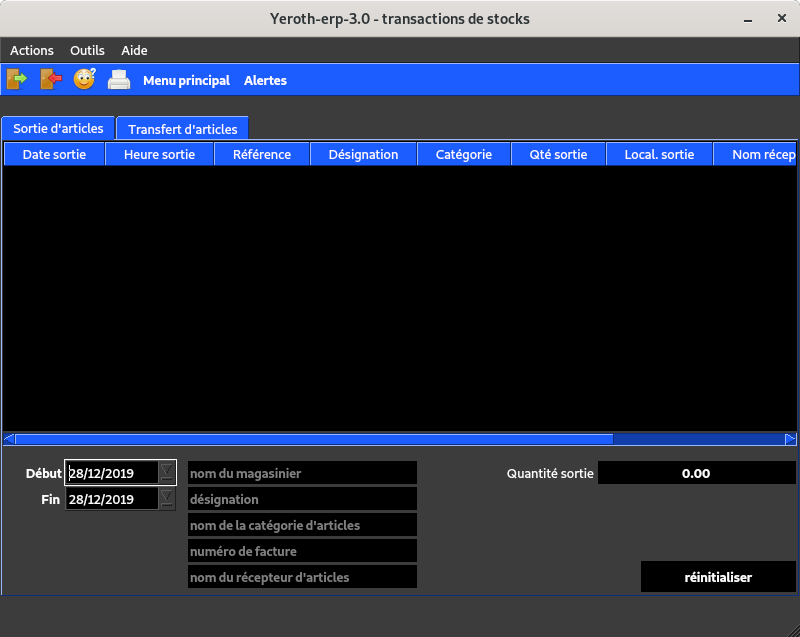
\includegraphics[scale=0.45]{images/yeren-transactions.png}
	\caption{La fen\^etre pour visualiser les sorties et les
		transferts d'articles.}
	\label{fig:yeren-transactions}
\end{figure}

La figure~\ref{fig:yeren-transactions} illustre
l'interface de \yeren pour visualiser les sorties et les
transferts d'articles.

Dans \yeren, une transaction est:
\begin{enumerate}[1)]
	\item une \textbf{sortie de stocks},
	\item ou bien un \textbf{transfert de stocks}.\\
\end{enumerate}

Une \textbf{sortie de stocks} est le retrait d'articles
par un client aupr\`es d'une boutique ou d'un d\'ep\^ot
de l'entreprise qui utilise \yeren.

Un \textbf{transfert de stocks} est un mouvement de stocks
d'une boutique ou d'un d\'ep\^ot de l'entreprise vers une
boutique ou d\'ep\^ot de votre entreprise.

%--------------------------------------------------------------

\nxsection{Voir les transactions sur une p\'eriode de temps}
\index{voir les transactions sur une p\'eriode de temps}

\begin{enumerate}[1)]
	\item S\'electionnez les dates de d\'ebut et de
	fin respectivement dans les champs de dates
	'D\'ebut' et 'Fin'.
\end{enumerate}

Les transferts de stocks s'affichent automatiquement
dans le $1^{\text{er}}$ premier onglet, pendant que
les sorties de stocks s'affichent automatiquement
dans le $2^{\text{\`eme}}$ onglet.	

L'utilisateur peut aussi ajouter les param\`etres suivants
\`a sa requ\^ete :

\begin{enumerate}[1)]
	\item le nom d'un magasinier (champs de texte 
	'\textbf{Magasinier}')
	\item la d\'esignation d'un l'article 
		(champs de texte '\textbf{D\'esignation}')
	\item la cat\'egorie d'un l'article 
		(champs de texte '\textbf{Cat\'egorie}')
	\item le num\'ero d'un bon de sortie 
		(champs de texte '\textbf{Num\'ero du bon de sortie}')
	\item le nom d'un r\'ecepteur
		(champs de texte '\textbf{Nom du r\'ecepteur}').
\end{enumerate}

Lorsque plus d'un param\`etre est utilis\'e pour
la requ\^ete, \yeren emploi l'op\'erateur logique
'\textbf{AND}' entre les diff\'erents param\`tres
pour g\'en\'erer le r\'esultat de la requ\^ete.

%--------------------------------------------------------------

\nxsection{Voir les transactions d'un magasinier}
\index{voir les transactions d'un magasinier}

\begin{enumerate}[1)]
	\item S\'electionnez dans le champs de texte
	'\textbf{Magasinier}' le nom du magasinier dont
	vous souhaitez observer les transactions effectu\'ees .
	
	\item Les transactions du magasinier choisi
	s'affichent automatiquement.
\end{enumerate}

%--------------------------------------------------------------

\nxsection{Voir les transactions d'un article}
\index{voir les transactions d'un article}

\begin{enumerate}[1)]
	\item S\'electionnez dans le champs de texte
	'\textbf{D\'esignation}' la d\'esignation de
	l'article dont vous souhaitez visualiser les
	transactions effectu\'ees .
	
	\item Les transactions de l'article choisi
	s'affichent	automatiquement.
\end{enumerate}

%--------------------------------------------------------------

\nxsection{Voir les transactions d'une cat\'egorie d'articles}
\index{voir les transactions d'une cat\'egorie d'articles}

\begin{enumerate}[1)]
	\item S\'electionnez dans le champs de texte
	'\textbf{Cat\'egorie}' le nom de la cat\'egorie
	d'articles dont	vous souhaitez visualiser
	les transactions effectu\'ees. 
	
	\item Les transactions de la cat\'egorie
	d'articles choisie s'affichent automatiquement.
\end{enumerate}

%--------------------------------------------------------------

\nxsection{Voir les transactions d'un bon de sortie}
\index{voir les transactions d'un bon de sortie}

\begin{enumerate}[1)]
	\item S\'electionnez dans le champs de texte
	'\textbf{Num\'ero du bon de sortie}' le num\'ero
	du bon de sortie dont vous souhaitez visualiser
	les transactions effectu\'ees.
	
	\item Les transactions du bon de sortie choisi
	 s'affichent automatiquement.
\end{enumerate}

%--------------------------------------------------------------

\nxsection{Voir les transactions d'un r\'ecepteur d'articles}
\index{voir les transactions d'un r\'ecepteur d'articles}

\begin{enumerate}[1)]
	\item S\'electionnez dans le champs de texte
	'\textbf{Nom du r\'ecepteur}' le nom de la
	personne dont vous souhaitez visualiser
	les transactions effectu\'ees, dont il a \'et\'e
	le r\'ecepteur.
	
	\item Les transactions de la personne choisi
	s'affichent automatiquement.
\end{enumerate}

%--------------------------------------------------------------

\nxsection{Imprimer le journal des transactions au format PDF}
\index{imprimer le journal des transactions au format PDF}

Il existe deux m\'ethodes pour imprimer 'le journal des
transactions' qui appara\^it dans la fen\^etre titr\'ee
'\textbf{Yeren - transactions}'.

\begin{itemize}[\mycheckmark{purplish}]
	\item \textcolor{purplish}{$\mathbf{1^{\text{\`ere}}}$ \textbf{m\'ethode}}\\
		Cliquez sur le lien
		'\textbf{Imprimer le journal des sorties/transferts}'
		qui se trouve dans le menu d\'eroulant '\textbf{Outils}'.\\

	\item \textcolor{purplish}{$\mathbf{2^{\text{\`eme}}}$ \textbf{m\'ethode}}\\
		Pressez simultan\'ement les boutons \bouton{CTRL}
		et \bouton{P} de votre clavier.
\end{itemize}

Un fichier au format PDF est alors g\'en\'er\'e et affich\'e.

\begin{figure}[!htbp]
	\centering
	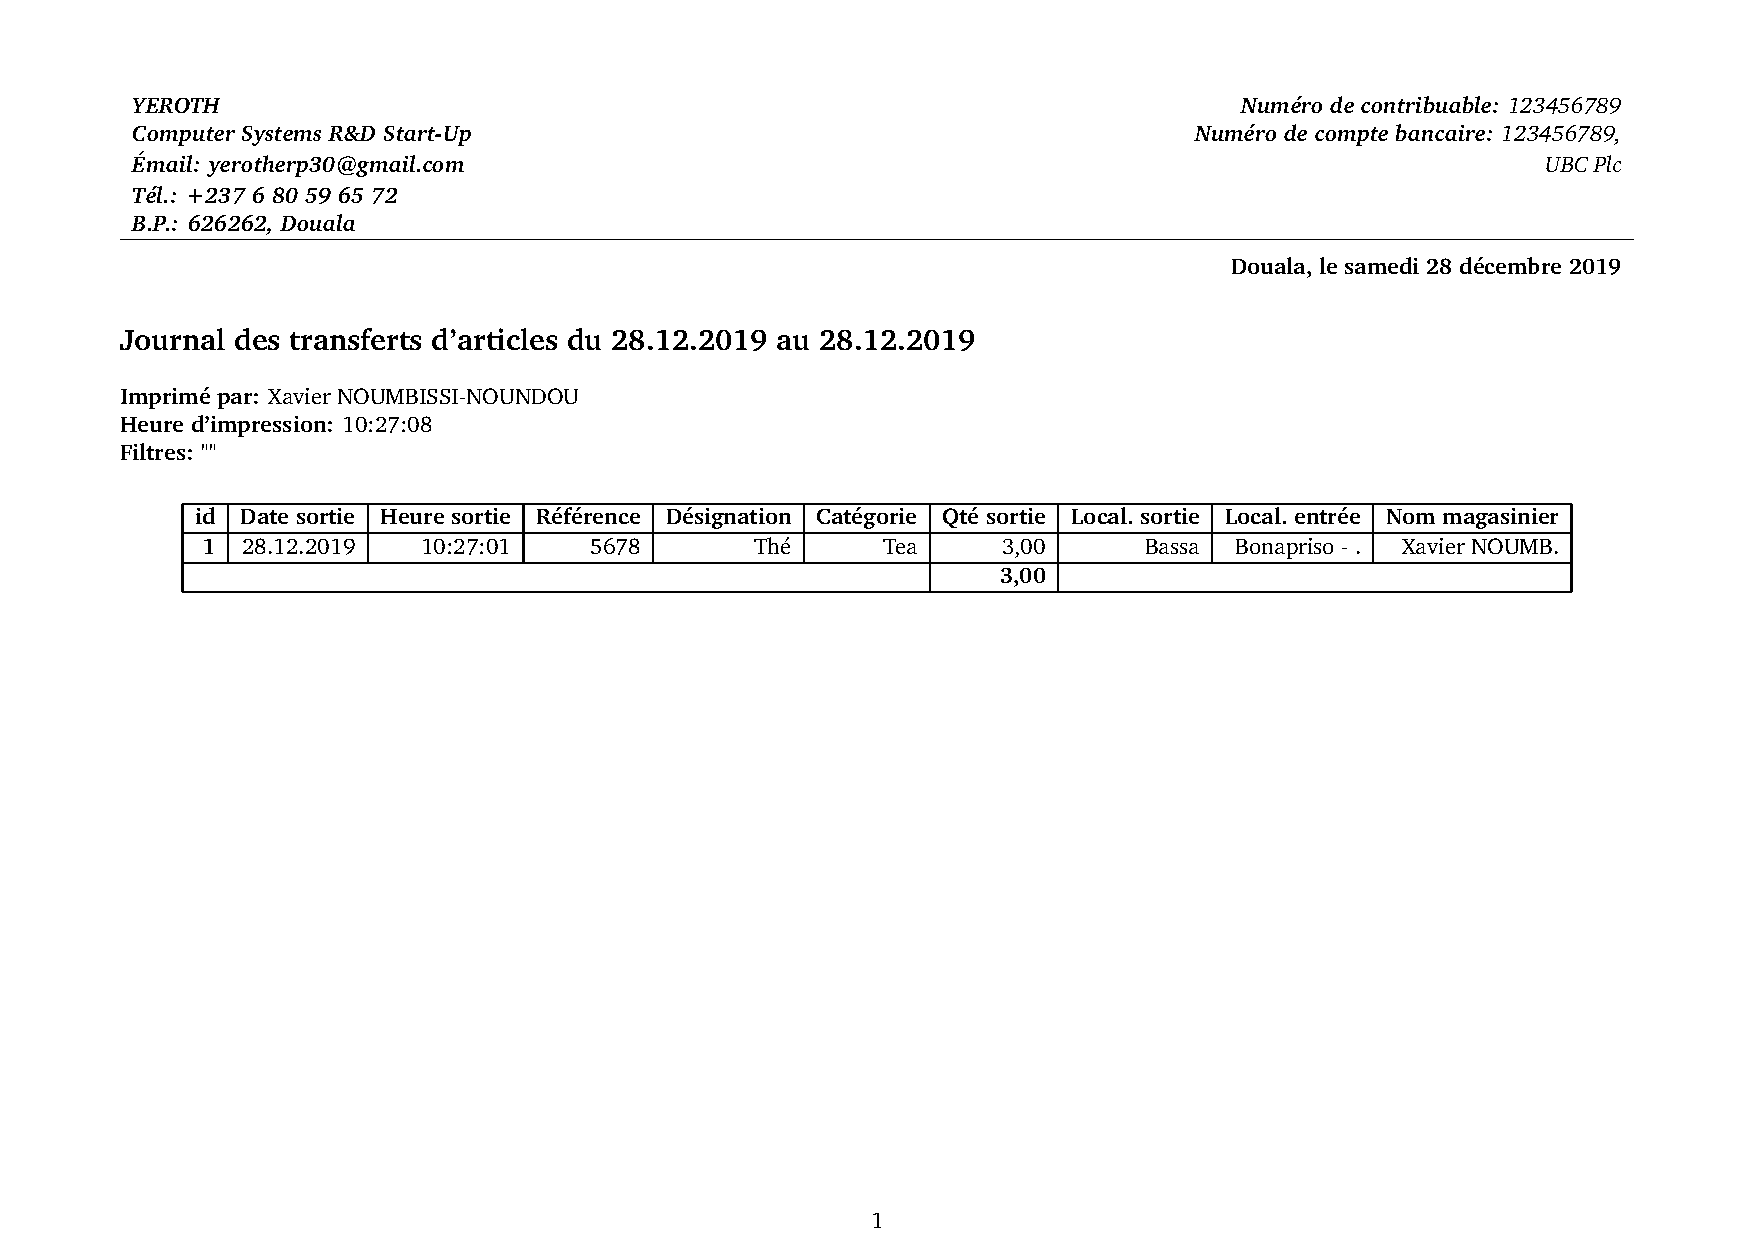
\includegraphics[scale=0.55]{images/yeren-journal-sortie-stocks-2017-06-14.pdf}
	\caption{Un journal de sorties des stocks.}
	\label{fig:yeren-journal-sorties-des-stocks}
\end{figure}

La figure~\ref{fig:yeren-journal-sorties-des-stocks} illustre un
exemple de journal de sorties des stocks au format PDF.

%--------------------------------------------------------------
